\documentclass[varwidth=true,border=2pt]{standalone}
\usepackage{circuitikz}

\begin{document}
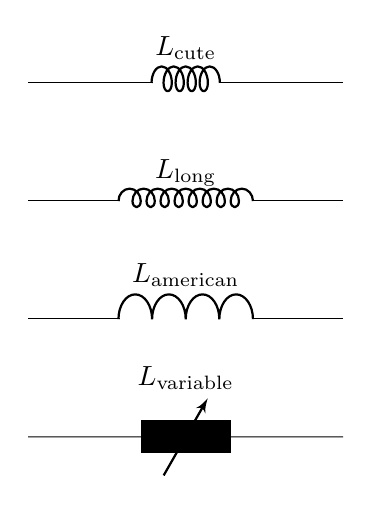
\begin{tikzpicture}
  % Adapted from the TeX Live circuitikz manual's inductor-style example.
  \draw (0,1.5) to[L,l=$L_{\mathrm{cute}}$] ++(4,0);
  \draw (0,0) to[cute inductor, inductors/scale=.75,
    inductors/width=1.6, inductors/coils=9, l=$L_{\mathrm{long}}$] ++(4,0);
  \ctikzset{inductor=american, inductors/scale=1.5}
  \draw (0,-1.5) to[L,l=$L_{\mathrm{american}}$] ++(4,0);
  \ctikzset{inductor=european, inductors/scale=1}
  \draw (0,-3) to[vL,l=$L_{\mathrm{variable}}$] ++(4,0);
\end{tikzpicture}
\end{document}
